\chapter{水电解质紊乱}

\section{前沿学术综述}

水是机体含量最多而又重要的组成成分,具有以下重要的生理功能:①体内一切生化反应进行的场所;②良好的溶剂,有利于营养物质及代谢产物的运输;③维持产热与散热的平衡,对体温调节起重要的作用。

水与溶解在其中的物质共称为体液,占体重的百分比因年龄、性别等而异。成年男性体液总量约占体重的60%,女性因皮下脂肪较丰富,约占体重50%,老年人约为45%,新生儿最高,为75%。体液不仅构成细胞生存的环境,同时也是细胞本身必不可少的成分。体液的组成相对恒定是所有细胞正常活动的前提。

细胞膜将体液分隔成细胞内液(约占体液的2/3)和细胞外液(约1/3)。细胞外液又分为组织间液(约占体重15%)、血浆(约占体重5%)和穿细胞液(约占体重2%)。绝大多数组织间液能迅速和血管内或细胞内液体进行交换,对于维持机体的水和电解质平衡,发挥巨大的作用,故称为功能性细胞外液。存在于结缔组织、软骨和骨质中的水分虽然也属于细胞外液,但由于与细胞内液的交换十分缓慢,称为非功能性细胞外液,生理情况下临床意义不大。

正常人体内组织间液和血浆内水的分布是复杂的,疾病状态下更是如此,如平时含水量极低的部位如腹腔或胸膜腔疾病状态下会表现为水肿(组织间隙容量增加)或液体潴留。一般来说,血管内容量的维持主要依靠以下几方面:①局限在血管内的大分子物质产生的胶体渗透压;②淋巴液从组织间隙回流入血管内腔;③组织间隙的静水压。相反的因素包括:①心脏和循环所产生的血管内静水压,促使液体由血管内向组织间隙转移;②组织间液的胶体渗透压,试图将血管内腔的液体拉出来。血管内容量决定了循环容量是否充分,同样,也影响了维持器官功能所需要的氧、营养和其他物质转运。

体液中的电解质指在体液中离解为带一个或多个电荷的离子,主要包括K\textsuperscript{+}
、Na\textsuperscript{+} 、Ca\textsuperscript{2+}
、Mg\textsuperscript{2+} 、Cl\textsuperscript{-}
、\ce{HCO3-}
、\ce{HPO3^2-}
和\ce{SO4^2-}
等。细胞内的主要溶质是钾离子和\ce{HPO3^2-}
,细胞外的主要溶质则是钠离子、Cl\textsuperscript{-}
和\ce{HCO3-}
。钠离子和钾离子沿着浓度梯度借助于细胞膜上的Na\textsuperscript{+}
-K\textsuperscript{+}
-ATP泵进行主动运输,维持浓度稳定。电解质的主要功能为:①维持体液的渗透压平衡和酸碱平衡;②维持神经、肌肉和心肌细胞的静息电位,并参与其动作电位的形成;③参与新陈代谢和生理功能活动。

体液的正常容量和分布、正常渗透压和各种电解质的正常含量,是保证细胞代谢活动正常进行和维持器官功能的必要条件。临床上多种疾病可引起水、电解质紊乱,进而使全身器官系统,特别是心血管、神经系统的功能紊乱。因此,了解水和电解质紊乱的发生机制及其演变规律,对临床防治水、电解质紊乱非常重要。

重症患者病情危重而复杂多变,虽严密监护并频繁地检测血电解质,但电解质紊乱的发生率仍很高
\protect\hyperlink{text00025.htmlux5cux23ch1-24}{\textsuperscript{{[}1{]}}}
。Michael等报道重症医学科内约50%的低钠血症在发病后24小时,甚至到72小时才被发现和处理。有报道显示,在美国住院患者中高钠血症的发病率为1%,而重症医学科住院患者的发病率较高------Polderman等研究发现,在重症医学科内发生高钠血症(重症医学科获得性高钠血症)的患者比例达5.7%,明显高于普通住院患者。患者一旦发生高钠血症,病情的观察和治疗都十分困难,如果对高钠血症的病因和病情演变缺乏正确的认识,纠正高钠血症的治疗不但无效,还可能恶化病情。

患者若合并高钠血症,其病死率相当高。普通住院患者高钠血症病死率为10%~60%,而危重病患者急性高钠血症病死率达42%~75%,远高于重症医学科所有患者的病死率(20%),且高钠血症的病死率与血钠水平直接相关。有研究显示,血钠高于160mmol/L的危重病患者病死率超过75%,另外,高钠血症的致残率也很高,很多患者遗留永久性神经功能障碍。

有研究显示,高钠血症的发生率和持续时间可以反映该重症医学科的治疗和监护水平。因此对重症医学科内常见可能发生电解质紊乱的患者进行严密监护,早期发现并进行积极合理的治疗是必须的。纠正电解质紊乱需要医生掌握电解质紊乱的病理生理变化,结合自己的经验,并根据患者对治疗的反应实施个体化治疗。

\section{临床问题}

\subsection{水钠代谢}

\subsubsection{细胞内外阳离子和阴离子的分布相同吗?}

体内主要的电解质有K\textsuperscript{+} 、Na\textsuperscript{+}
、Ca\textsuperscript{++} 、Mg\textsuperscript{2+}
、Cl\textsuperscript{-} 、\ce{HCO3-}
、\ce{HPO3^2-}
和\ce{SO4^2-}
等。细胞外液主要阳离子是Na\textsuperscript{+}
,主要阴离子是Cl\textsuperscript{-}
和\ce{HCO3-}
;细胞内液中主要阳离子是K\textsuperscript{+}
,主要阴离子是\ce{HCO3^2-}
。不同部位体液中电解质的组成及各自的浓度并不相同,但在正常情况下,均处于动态平衡,保持相对稳定(表\ref{tab19-1})。

\begin{table}[htbp]
\centering
\caption{体液中主要电解质含量}
\label{tab19-1}
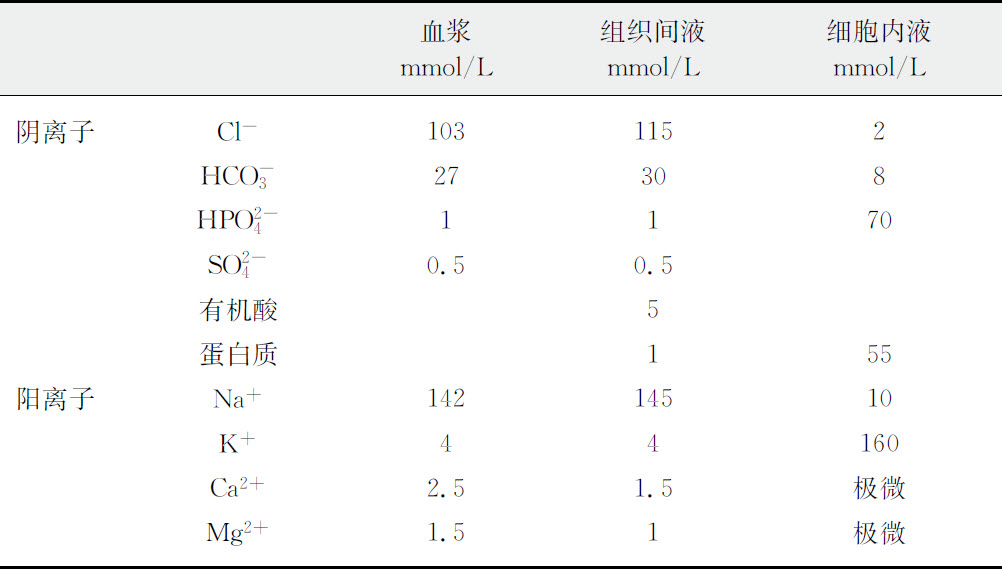
\includegraphics{./images/Image00159.jpg}
\end{table}

\subsubsection{血浆渗透压的主要决定因素有哪些?}

渗透压指的是高浓度溶液所具有的吸引和保留水分子的能力,其大小与溶液中所含溶质颗粒数目成正比而与溶质的分子量半径等特性无关。血浆的渗透压主要来自溶解于其中的晶体物质,特别是电解质,另一部分来自于蛋白质。

由晶体物质所形成的渗透压称为晶体渗透压,它的80%来自Na\textsuperscript{+}
和Cl\textsuperscript{-}
,与组织液的晶体渗透压基本相等。由于晶体物质颗粒质量很小,粒子数目比胶体多,故血浆渗透压主要取决于晶体离子,尤其是Na\textsuperscript{+}
浓度。

由蛋白质所形成的渗透压称为胶体渗透压,由于组织液中蛋白质很少,所以血浆的胶体渗透压高于组织液的胶体渗透压。血浆胶体渗透压主要来自白蛋白。血浆胶体渗透压对于维持血管内外的水平衡极为有重要,其正常范围在280~310mOsm/kg,低于280mOsm/kg为低渗,高于310mOsm/kg为高渗。

\subsubsection{决定组织水肿的重要因素有哪些?}

过多的液体在组织间隙或体腔内积聚称为水肿。水肿不是一个独立的疾病,而是与某些疾病相伴随的病理过程。

水肿可发生于局部,称局部水肿,如肺水肿、脑水肿;也可波及全身,称全身性水肿,如充血性心力衰竭时的心性水肿、肾病或肾炎时的肾性水肿、肝脏疾病时的肝性水肿和营养不良时的营养不良性水肿等;另外还有的全身性水肿至今原因不明,称“特发性水肿”。

水肿发生的部位虽然各有差别,但其发生机理是基本相同的。正常情况下,组织间隙液体的量是相对恒定的。这种恒定的维持,是有赖于血管的内外液体和体内外液体交换的平衡。水肿的发生就是由某些疾病引起的这两方面的平衡障碍所造成,由多种原因引起。

水肿的发病机制主要有如下。

(1)血管内外液体交换平衡失调 正常情况下,组织液的产生和回流保持动态平衡,这种平衡主要的影响因素有有效静水压、有效胶体渗透压和淋巴回流等几个因素:①驱使血管内液体向外滤出的力量是有效静水压,毛细血管内平均静水压为20mmHg,组织间隙静水压为-10mmHg,两者之差为30mmHg,即为有效静水压。②促使液体回流至毛细血管内的力量是有效胶体渗透压,正常人血浆胶体渗透压为25mmHg,组织间液的胶体渗透压为15
mmHg,两者之差10mmHg为有效胶体渗透压。③促使组织液形成的压力称为有效滤过压,有效滤过压=(组织间隙胶体渗透压+毛细血管内静水压)-(毛细血管内胶体渗透压+组织间隙静水压),正常情况下血管内外液体交换处于动态平衡。④淋巴回流,组织液回流剩余的部分须经淋巴系统回流进入血液循环,组织间隙静水压升高时,淋巴液生成速度加快;另外,淋巴管壁的通透性较高,蛋白质易通过,因此,淋巴回流不仅可把略多生成的组织液送回体循环,而且可以把漏出的蛋白质、大分子物质送回体循环。

上述任何因素失调均可使组织液生成增多,形成水肿。引起组织液生成大于回流的因素主要有以下几方面------①毛细血管血压增高:由于毛细血管血压增高,使液体从毛细血管滤出到组织间隙增多,而又阻碍液体回流入毛细血管,这样就造成组织液积聚过多,当其超过淋巴的回流代偿时,就出现水肿。如心力衰竭时引起的全身性水肿;肝硬变时引起的腹水,以及局部静脉受阻时引起的局部水肿等,基本原因之一,就是毛细血管血压增高。②血浆胶体渗透压降低:血浆胶体渗透压是使组织液回流到毛细血管的一种力量,当血浆胶体渗透压降低时,组织液生成增多,回流减少,组织间隙液体积聚过多,形成水肿。这种水肿常为全身性的。由于血浆胶体渗透压的高低主要取决于血浆蛋白含量,尤其是白蛋白含量。因为白蛋白量多、分子小、吸水力强、对渗透压影响极大,所以当血浆蛋白总量低于50g/L(正常为67~79g/L)或白蛋白含量低于25g/L(正常为38~48g/L)时,即可发生水肿。消化道疾病时消化吸收障碍,蛋白质摄取不足;肝功能不全时蛋白质合成减少;肾病综合征时蛋白质丧失过多等,都会引起水肿。③毛细血管通透性增加:正常毛细血管壁仅允许水分、晶体物质(如Na\textsuperscript{+}
、葡萄糖等)和少量白蛋白通过。但在病理情况下,通透性增加,会使大量蛋白质漏出到组织液中。结果,一方面血管内液体渗透压降低,另一方面组织液胶体渗透压升高,结果则发生水肿。炎症引起的水肿,就是因毛细血管通透性增加所致。④淋巴回流受阻:组织液除了大部分从毛细血管静脉端回流外,少部分还从淋巴管回流入血。当淋巴管阻塞,淋巴回流受阻时,就可使含蛋白质的淋巴液在组织间隙中积聚而引起水肿,称为淋巴水肿。如恶性肿瘤细胞侵入并堵塞淋巴管;临床进行广泛摘除淋巴结的手术;丝虫病时,主要淋巴管道被成虫阻塞等,均可引起淋巴水肿。

(2)体内外液体交换障碍 正常人体主要通过肾的滤过和重吸收来调节水和钠盐的摄入量与排出量的动态平衡,从而保证体液总量和组织间液量相对恒定。正常情况下,通过肾小球滤过的水、钠,99%以上被肾小管重吸收,只有约1%从尿中排出。若肾小球滤过率和肾小管重吸收率保持这个比例,就不致发生水、钠潴留,称为肾小球肾小管平衡。任何原因使肾小球滤过率减少而肾小管重吸收率并未减少,或肾小球滤过率没有明显变化而肾小管重吸收明显增强,再或肾小球滤过率减少而肾小管重吸收增强同时出现,都会导致肾小球、肾小管平衡失调,从而引起水、钠排出减少,在体内潴留,成为全身性水肿形成的重要原因。①肾小球滤过率下降:造成肾小球滤过率下降的原因一是广泛的肾小球病变,如急性肾小球肾炎时,肾小球因内皮细胞肿胀和炎性渗出物堆积而阻碍过滤;慢性肾炎时,因肾单位破坏严重,滤过面积减少而导致肾小球滤过率下降等;二是有效循环血量减少,如心力衰竭、肾病综合征和肝硬变等,均可使有效循环血量减少。由于有效循环血量减少,通过颈动脉窦和主动脉弓压力感受器,反射性地引起肾脏小血管收缩,肾血流量更加减少,造成肾小球滤过率下降。②肾小管重吸收增强:这是引起水钠潴留全身性水肿的重要环节。造成肾小管重吸收增强的因素是多方面的。如醛固酮和抗利尿素增多,醛固酮由肾上腺皮质球状带分泌,在肝中被破坏,它能促进肾小管(主要是肾远曲小管)对钠的重吸收,因此,当醛固酮增多时,就能引起钠潴留。钠潴留又使血液中晶体渗透压增高,反射性地刺激垂体后叶增加抗利尿素分泌,抗利尿素有促进肾远曲小管和集合管对水重吸收的功能,这样便使过多的水潴留于体内。③远曲小管和集合管重吸收增加:远曲小管和集合管重吸收水钠受醛固酮和抗利尿激素等的调节。

\subsubsection{细胞外液不足和细胞外液过多的常见原因有哪些?}

细胞外液不足的常见原因有:①剧烈呕吐、腹泻是等张性体液容量不足最常见的原因。②大面积烧伤、腹膜炎、急性呼吸窘迫综合征及肠道梗阻时使大量体液渗出到第三间隙。③急性肾衰竭的多尿期。④长期连续使用利尿药。⑤肾上腺皮质功能不全如艾迪生病时醛固酮分泌不足等。这些情况均可引起肾脏丢失水分增多。

细胞外液过多的常见原因主要是钠和水成比例潴留在体内,导致细胞外液过多。体液容量过多常见于充血性心衰、肝硬化、肾病综合征、库欣综合征、低蛋白血症以及医源性过量输注生理盐水等。如液体存在血管内则称为高容量状态,液体转移到组织间隙则导致水肿。

\subsubsection{有效循环血量减少是否等同于细胞外液不足?}

细胞外液不足引起有效循环血量减少最常见,但有效循环血量减少还可伴有细胞外液正常或增加。细胞外液减少由细胞外液体丢失增加或补充不足引起,或两种因素同时存在。失血、呕吐、腹泻或通过皮肤的液体丢失过多(如出汗或烧伤)都可导致细胞外容量迅速减少。因肾性疾病致尿量明显增加后出现失水和失钠、肾上腺功能不全、利尿剂或高血糖症(渗透性利尿)等亦是导致细胞外液不足的常见原因。细胞外液不足还可由于液体补充不足引起,通常见于饮食不当或无法摄入足够水和溶质的患者。

细胞外容量正常的有效循环血量不足是由血管内外液体失衡所引起的。血管内胶体渗透压、静水压和血管的完整性是维持血管内容量稳定的重要因素。血管内胶体渗透压降低、静水压增高促进血管内液体向血管外移位;而炎症反应、感染、休克以及其他重症疾病增加血管通透性,导致血管内容量减少、组织间隙液体增加(如胸膜腔渗出或腹水)。上述均表现为细胞外容量正常的有效循环血量不足。

某些情况下,血管内升高静水压或胶体渗透压降低导致有效循环血量减少,机体作为代偿,继而会使得肾脏重吸收水钠增加,这会导致细胞外总容量增加。如肝硬化伴有低白蛋白血症出现腹水,是门脉高压和胶体渗透压降低共同作用的结果;心衰时静水压增高导致水肿;而肾病综合征患者由于胶体渗透压严重降低产生水肿等。因此,即使在细胞外容量明显增加的情况下也可出现有效循环血量的明显减少。

\subsubsection{低钠血症的临床表现、病因与发病机制是什么?}

低钠血症的临床表现是非特异性的。轻度低钠血症(血清钠浓度120~135mmol/L)主要有味觉减退、肌肉酸痛;中度低钠血症(血清钠浓度115~120mmol/L)有头痛、个性改变、恶心、呕吐等;重度低钠血症(血清钠浓度低于115mmol/L)则可出现昏迷、反射消失。导致低钠血症的主要原因有水过量或钠丢失。

(1)水过量 因水过量引起的低钠血症称为稀释性低钠血症,其特征为机体摄入水总量超过排出水量,以致水分在体内潴留,引起血浆渗透压降低和细胞外液容量增加。常见原因有:①肾功能不全,肾脏排水能力减低;②机体摄入水分过多或医源性输入过多液体,尤其是低渗液体;③有效循环血量减少或其他非渗透性刺激使抗利尿激素释放,导致低钠血症,这种情况临床上称为抗利尿激素异常分泌综合征。

导致抗利尿激素分泌增多的原因有:①下丘脑抗利尿激素生成增多,如中枢神经系统功能紊乱(如脑外伤、脑血管意外和脑部肿瘤);内分泌功能紊乱(如甲状腺功能紊乱、艾迪森病);外科术后(特别是心脏术后);②抗利尿激素病理性分泌过多,见于恶性肿瘤尤其是肺癌;③摄入抗利尿激素样药物,如血管加压素、催产素,尤其是和无钠液体一起静脉给药;④药物导致抗利尿激素释放增多或抗利尿激素对远端肾小管和集合管的作用增强,如口服降糖药物、三环抗抑郁药物、吗啡、胆碱能药物、抗惊厥药物、前列腺素抑制剂等。

(2)钠丢失 钠丢失导致的低钠血症称为短缺性低钠血症,其特征为细胞外液容量减少和钠丢失。钠丢失有经肾和肾外两种途径。经肾丢失钠多见于长期应用利尿剂而又低盐饮食者。肾外丢失常随体液丢失而发生,如呕吐、腹泻致大量的钠随消化液排出或肾上腺功能低下。

\subsubsection{重型颅脑外伤发生低钠血症的机制是什么?}

重型颅脑外伤患者常发生血钠代谢障碍,可以导致低钠血症或高钠血症。重型颅脑外伤引起的低钠血症见于:①脑性盐耗综合征;②抗利尿激素分泌不适当综合征;③尿崩症、渴感缺失或患者给水过多引起高容量性稀释性低钠血症;④过量的利尿剂引起肾脏排钠增加引起的低钠血症。低钠血症的主要表现是由脑水肿颅内压增高引起的神经功能失常。严重的低血钠或血钠水平的急剧下降将加重重型颅脑外伤患者意识障碍程度,使昏迷程度加深。目前认为抗利尿激素分泌不适当综合征和脑性盐耗综合征是重型颅脑外伤患者合并低钠血症的两种常见原因。

抗利尿激素分泌不适当综合征和脑性盐耗综合征的临床表现和生化检查极为相似,它们的主要区别在于细胞外液量的状态和钠代谢的状态。抗利尿激素分泌不适当综合征是因抗利尿激素分泌过多导致水潴留,使细胞外液量正常或稍高,钠代谢为正平衡;而脑性盐耗综合征是因肾脏对钠盐的吸收减少所致,主要特征是细胞外液的减少和钠的负平衡,目前认为脑性盐耗综合征的发生与脑部疾病后血清心房利钠肽、脑利钠肽等利尿钠因子的分泌紊乱及神经因素对肾功能的直接影响有关。两者虽然同为低钠血症,抗利尿激素分泌不适当综合征因水潴留而产生稀释性低钠血症,脑性盐耗综合征则是原发的尿排钠增多致钠盐减少而致的失钠性低钠血症,因此,两者治疗措施完全不同。在不存在低血压的情况下,测量中心静脉压有助于它们之间的鉴别诊断。在无法确诊时可以采用实验性限水治疗,脑性盐耗综合征限水治疗后低钠血症加重而抗利尿激素分泌不适当综合征限水治疗有效。脑性盐耗综合征的根本性治疗是补充容量和恢复钠的正平衡,这与抗利尿激素分泌不适当综合征的限水治疗截然相反。

\subsubsection{怎样把握纠正低钠血症的速度?}

低钠血症一旦确诊应立即静脉给予等张液体。总的原则是:输注速度应先快后慢,总输入量应分次完成。需要补钠的量由下面的公式计算(1g氯化钠中含Na\textsuperscript{+}
17mmol)。

\[
\text{补钠量(mmol)}=0.6(\text{女性}0.5)\times \text{体重(kg)}\times[\text{血钠正常值(mmol/L)}-\text{血钠实测值(mmol/L)}]    
\]

治疗必须遵守以下原则:首先,注意补钠的速度不宜过快,否则会导致细胞脱水,尤其是中枢神经系统并发症如脑桥中央髓鞘溶解(常发生在快速纠正低钠血症后的1~6天),其他的中枢神经系统并发症有痉挛性延髓性麻痹、四肢轻瘫、癫痫和运动障碍等。

急性或严重低钠血症患者以每小时提高血清钠水平1~2mmol/L的速度输注,但血清钠水平升高超过每小时0.5mmol/L的速度仅限于第一个48小时内。在开始治疗时可予3%的氯化钠溶液以每小时15~50ml的速度输注。慢性或很难估计病程的低钠血症患者血清钠水平提高应控制在每小时0.5mmol/L以内。建议每24小时血清钠水平升高应控制在8~12mmol/L,治疗时间以48~96小时为宜。第一个48小时血清钠水平的增高不能超过20~25mmol/L。

其次,治疗过程中密切监测血钠,早期应2~4小时检测一次血钠水平,直至症状消失,然后4~8小时检测一次,直到血清钠恢复至正常水平。

第三,避免发生高钠血症,在治疗过程中应防止血钠超过145mmol/L。

对于稀释性低钠血症患者,在控制原发病的同时,应限制饮水并适当利尿
\protect\hyperlink{text00025.htmlux5cux23ch1-24}{\textsuperscript{{[}1{]}}}
。

\subsubsection{高钠血症的病因和临床表现有哪些?}

高钠血症是指血清钠浓度超过150mmol/L,其常见病因如下。

(1)水的丢失超过钠的丢失 机体丢失低渗体液,如在发热、过度换气和暴露于高温环境时经呼吸道和皮肤丢失。另外,严重腹泻、呕吐亦可经胃肠道丢失大量低渗体液。

(2)中枢神经系统疾病 这类疾病可影响抗利尿激素的分泌或其对肾脏的作用,削弱肾脏重吸收水的能力,导致肾脏排水多于排钠。渗透性利尿也会使肾脏失水多于失钠。丢失大量低渗液体后,如不能及时补充,可发生伴有细胞外液容量不足的高钠血症。此外有研究报道,下丘脑损害可导致促肾上腺激素释放激素的异常分泌,并兴奋醛固酮分泌而保钠排钾,使血钠增高。

(3)钠的摄入超过水的摄入 因摄入过多导致的高钠血症较少见。可见于意外大量口服食盐或海水,医源性因素包括静脉大量输注含钠液体。

高钠血症时细胞外液容量可基本正常,也可伴有细胞外液容量减少,或细胞外液容量增多的情况。

高钠血症可出现在任何年龄阶段,临床症状可能不典型,如乏力、唇舌干燥、皮肤失去弹性、烦躁不安,甚至躁狂、幻觉、谵妄和昏迷,高钠血症导致的脑萎缩可引起脑出血、蛛网膜下腔出血,严重者可致死亡。中枢神经功能异常是高钠血症最主要的临床表现,常与危重患者的症状、体征相重叠,大多数情况不好区分,但血钠浓度是病情严重程度的一个指标,血钠浓度越高、增高越快,上述症状就会越明显,患者病情越重。

\subsubsection{重型颅脑外伤时高钠血症的发病原因是什么?}

重型颅脑外伤高钠血症发病率高,对脑病理生理影响大,死亡率高达42%~75%,应予以重视,其发生原因包括:①严重颅脑外伤患者因使用大剂量脱水药物、高热、大量出汗、气管切开经呼吸道失水明显增加等原因,使液体出量大于入量或过分的液体限制引起低容量性高钠血症;②因给予过多的高渗盐而引起高容量性高钠血症;③下丘脑损伤导致渴觉中枢和(或)渗透压感受器损伤,血浆渗透压的升高不能引起渴感饮水和(或)抗利尿激素(ADH)释放,但抗利尿激素对非渗透压刺激反应正常导致高钠血症;④机体处于应激状态,醛固酮分泌增加,导致水钠潴留;⑤部分患者血糖常较高,可产生渗透性利尿,加重高钠血症。

\subsubsection{如何纠正高钠血症及注意事项?}

高钠血症的治疗原则是治疗原发病,防止水继续丢失和纠正低血容量。合适治疗的前提是正确评估高钠血症患者的容量状态,如有效循环血量是否过多?有效循环血量是否不足?应及时了解血钠升高的水平、升高的速度及高钠血症持续的时间。早期一旦发现高血钠,应立即停用一切含钠液体,改输注低渗液体(0.45%或0.225%的氯化钠溶液)或低分子右旋糖苷。水的需要量按下面公式计算:

\[
\text{水补充量(ml)}=4\times \text{体重(kg)}\times[\text{血钠实测值(mmol/L)}-\text{血钠正常值(mmol/L)}]    
\]

计算所得的补水量不宜在当日一次输入,一般可分在2~3天内补给。若病情允许应停用高渗利尿剂。肾功能障碍者必要时可行血液透析治疗。

对有症状的急性高钠血症,可快速予以纠正,快速纠正能改善预后而不增加脑水肿危险,但由于血清钠上升过快,脑细胞尚未适应这种不平衡状态,因此这类患者血清钠水平每小时降低1~2mmol/L是适当的。但在血清钠水平已经下降20~25mmol/L或血清钠水平已经降至148mmol/L以下等情况时应停止快速纠正。

发病时间较长或发病时间不明确时应减慢血清钠下降的速度,以预防惊厥、脑水肿、膨出,甚至脑疝的发生。这些患者血钠浓度下降速度最大不超过每小时0.5mmol/L,以每24小时下降10~12mmol/L为宜。若患者出现有效循环血量不足或低血压时建议可以用生理盐水、复方氯化钠溶液、乳酸钠林格注射液、低渗液体(0.45%或0.225%的氯化钠溶液)或低分子右旋糖苷扩容,尽快纠正不稳定的血流动力学状况。

治疗过程中密切监测血清钠水平,早期应2~4小时检测一次血钠水平,直至症状消失;然后每4~8小时检测一次,直到血清钠降低到145mmol/L
\protect\hyperlink{text00025.htmlux5cux23ch1-24}{\textsuperscript{{[}1{]}}}
。

\subsection{钾的代谢}

\subsubsection{人体内钾的分布与代谢是怎样的?}

钾是生命必需的电解质之一,其生理作用包括维持细胞新陈代谢、调节渗透压和酸碱平衡、保持细胞应激功能等。人体每天摄入大约100mmol的钾,肾脏排泄90%,剩余的由胃肠道排泄。钾主要储存在细胞内,血清钾仅占机体总钾的2%,血清钾浓度为3.5~5.5mmol/L;细胞内钾占98%,浓度高达160mmol/L。细胞内和细胞外液中钾离子浓度差异巨大,是形成神经肌肉细胞膜静息电位的主要因素。因此,很小的细胞外钾离子浓度异常,即可导致危及生命的并发症。

限制钾细胞内外转移的主要因素为细胞膜上的Na\textsuperscript{+}
-K\textsuperscript{+}
-ATP泵,以维持细胞内很高的钾浓度。此泵的活性受下列因素的影响:胰岛素、胰高血糖素、激素、醛固酮、β肾上腺素兴奋剂、酸-碱平衡紊乱等。

低钾血症是指血清钾浓度低于3.5mmol/L,而当血清钾浓度超过5.5mmol/L时称为高钾血症。很多时候血清钾浓度不能真正反映细胞内钾的水平,亦不能代表人体内总钾的多少。因此,低钾血症时并不代表着患者体内总钾的缺失,但临床医生仍然只能依照血清钾水平来决定是否需要补充钾及补钾的剂量。通常估计血清钾每下降0.3mmol/L,体内总钾约丢失100mmol
\protect\hyperlink{text00025.htmlux5cux23ch1-24}{\textsuperscript{{[}1{]}}}
。

\subsubsection{低钾血症的常见病因和临床表现有哪些?}

危重病患者病情复杂,治疗措施多,经常会发生低钾血症,常见的低钾血症病因如下。

(1)摄入减少 长期不能进食而又没有静脉补充足够的钾,此时尽管钾摄入减少,但肾脏仍持续排泄钾,从而造成钾丢失。

(2)排出增多 ①消化道丢失:腹泻、呕吐、持续胃肠减压等导致大量富含钾的消化液丢失,呕吐造成的代谢性碱中毒也可使肾脏排钾增多。②经肾脏失钾:长期或大量使用排钾利尿剂;急性肾衰竭的多尿期;Ⅰ型肾小管酸中毒时由于远曲小管泌H\textsuperscript{+}
障碍,K\textsuperscript{+} -Na\textsuperscript{+}
交换增多而导致尿钾增多;盐皮质激素过多时肾脏远曲小管和集合管K\textsuperscript{+}
-Na\textsuperscript{+}
交换增多导致钾排除增多;一些药物如顺铂和两性霉素B可通过影响肾小管而使肾丢失钾。

(3)钾从细胞外向细胞内转移 ①碱中毒时H\textsuperscript{+}
从细胞内溢出,相应量的钾转移到细胞内;②输注葡萄糖和胰岛素,胰岛素促进细胞合成糖原,需要钾参与,细胞外的钾随葡萄糖进入细胞内;③甲状腺素周期性麻痹可能与甲状腺素增强Na\textsuperscript{+}
-K\textsuperscript{+} -ATP酶活性,使钾向细胞内转移有关。

低钾血症的临床表现是多样的,最危及生命的症状包括心脏传导系统和神经肌肉系统。轻度低钾血症的心电图表现是T波低平或消失,并出现U波,严重低钾血症可导致致命性的心律失常如室性心动过速、室性纤颤或猝死
\protect\hyperlink{text00025.htmlux5cux23ch2-24}{\textsuperscript{{[}2{]}}}
。在神经肌肉系统,低钾血症最突出的症状是骨骼肌弛缓性瘫痪和平滑肌失去张力、横纹肌溶解,累及呼吸肌则导致呼吸衰竭。低钾血症也可产生胰岛素抵抗或胰岛素释放受阻,导致明显的糖耐量异常。钾排泄减少导致肾脏的尿浓缩能力下降,出现多尿和低比重尿。

\subsubsection{低钾血症的治疗原则及其注意事项是什么?}

低钾血症的治疗原则为积极处理原发病,对症处理,补钾,避免高钾血症。

补钾原则为轻度低钾血症,无临床表现者口服补钾,分次给予40~80mmol/天;严重低钾血症患者(胃肠道不能利用、K\textsuperscript{+}
<2.0mmol/L或有威胁生命的症状)应立即静脉补钾。初始补钾的速度一般认为10~20mmol/小时是比较安全的,有报道认为在监测的条件下,静脉给钾的速度可达40mmol/小时。若严重低钾伴威胁生命的临床表现,可在短时间内补钾40~80mmol,但需注意的是:

(1)应严密监测血K\textsuperscript{+}
水平,补钾60~80mmol或给予补钾后1~4小时内应复查血钾水平。

(2)若补钾的速度超过10mmol/小时应持续心电监护,密切观察心电图的变化,严防威胁生命的高钾血症发生。

(3)在肾功能障碍患者补钾的速度减为肾功能正常患者的50%。

(4)一般认为每日补钾量不宜超过100~200mmol,Michael等报道对于严重低钾患者每日总补钾量可达240~400mmol,但须密切监测血清钾的水平,防止高血钾的发生。

(5)外周静脉输注高浓度钾会刺激静脉壁,产生疼痛和静脉炎,一般认为经外周静脉补钾浓度不应超过40mmol/L。Michael等建议经外周静脉补钾的钾的浓度不超过80mmol/L,超过120mmol/L必须经中心静脉输注。

(6)用氯化钠溶液稀释含钾液体,不建议用葡萄糖或低分子右旋糖苷
\protect\hyperlink{text00025.htmlux5cux23ch1-24}{\textsuperscript{{[}1{]}}}
。

\subsubsection{高钾血症的病因与发病机制有哪些?}

高钾血症是由于摄入增加或排出减少,或由于细胞内钾离子向细胞外转移造成的。

(1)摄入增多 在肾功能正常的情况下,高钾饮食一般不会引起高钾血症,只有在静脉补充钾过多过快,特别是肾功能低下时,才可能引起高钾血症。

(2)排出减少 是引起高钾血症的主要原因,常见于以下情况:①肾衰竭,急性肾衰竭少尿期和慢性肾衰竭的少尿或无尿期,由于肾小球滤过率下降和肾小管排钾功能障碍,可发生高钾血症;②盐皮质激素缺乏,醛固酮分泌减少或作用减弱时,肾远曲小管和集合管对钾的排泄降低,发生高钾血症,见于艾迪森病、肾上腺皮质激素合成所需要的酶缺乏、使用血管紧张素转换酶抑制剂类药物等情况;③原发性肾小管泌钾障碍,见于IV型肾小管酸中毒,是由于远曲小管对钾的分泌障碍造成的。

药物:保钾利尿剂抑制远曲小管和集合管对钾的分泌,洋地黄类药物抑制细胞膜Na\textsuperscript{+}
-K\textsuperscript{+} -ATP酶,造成高钾血症。

(3)细胞内钾离子向细胞外大量转移 可能发生在细胞大量分解、酸中毒、组织缺氧、家族性高钾性周期性麻痹和胰岛素缺乏等情况。

\subsubsection{高钾血症典型的临床表现和治疗原则是什么?}

高钾血症主要影响心脏和神经肌肉的传导,故典型的临床表现有:严重的心动过缓、房室传导阻滞甚至窦性停搏。轻度高钾血症(5.5~6.0mmol/L)时心电图表现为T波高尖;而血钾继续升高时,PR间期延长,P波消失,QRS波增宽,最终心脏停跳。对于神经肌肉来说,高钾血症的表现与低钾血症非常类似,包括骨骼肌和平滑肌的无力、麻痹。

高钾血症一旦确诊,必须立即治疗。

(1)促进钾的排泄 应用呋塞米或其他袢利尿剂治疗可以使肾脏发挥最大排钾作用。口服或直肠应用小剂量聚苯乙烯磺酸钠可以排出钾。严重威胁生命的高钾血症(血清钾>6.5mmo/L)需要行血液透析治疗。

(2)使钾转移到细胞内 ①通过钙来改变自律细胞的兴奋性,能够立即保护心脏免受高钾血症对传导系统的损害,一般给予10%葡萄糖酸钙静脉注射。②10%葡萄糖加入普通胰岛素配成10μ/L的溶液以250~500ml/小时速度静脉滴注。③输注碳酸氢钠纠正酸中毒。具体药物的剂量、给药途径、起效时间和药物维持时间见表\ref{tab19-2}
\protect\hyperlink{text00025.htmlux5cux23ch1-24}{\textsuperscript{{[}1{]}}}
。

\begin{table}[htbp]
\centering
\caption{高钾血症的药物治疗}
\label{tab19-2}
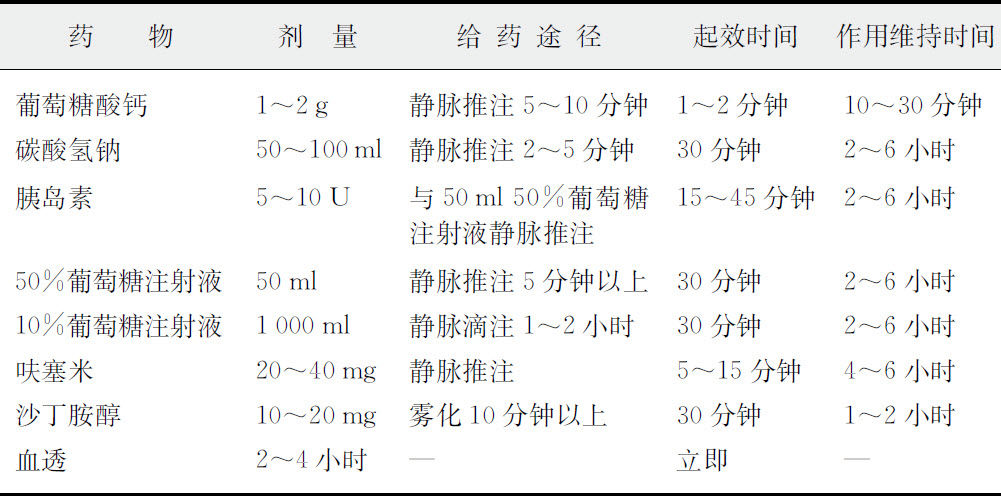
\includegraphics{./images/Image00162.jpg}
\end{table}

\subsection{钙磷的代谢}

\subsubsection{钙磷的代谢途径及其调节机制是什么?}

钙和磷是人体内含量最丰富的无机元素。在正常成人,钙约占体重的1.5%,99%的钙和86%的磷以羟磷灰石的形式存在于骨和牙齿当中,其余分布于体液和软组织中,以溶解状态存在。钙和磷的代谢在许多方面是相互联系的,机体从食物中摄取钙和磷、又把它们从尿和粪中排泄,成人每日摄取和排泄量大致相等,处于动态平衡之中。

血钙指血浆中所含的钙,可分为非离子化钙和离子钙。非离子化钙是指与血浆蛋白(主要为白蛋白)结合的钙(约占体内总钙量的50%)及与柠檬酸或其他酸结合的钙(占5%),它们不易透过毛细血管壁;离子化钙(约占体内总钙量的45%)主要为游离钙离子及少量的可溶性钙盐。在血浆中发挥生理作用的主要为游离钙离子,维持着神经肌肉的稳定性。血浆中非离子化钙和离子钙的比例呈动态平衡关系,此平衡受血浆pH影响,血液偏酸时,游离钙离子浓度升高;相反,血液偏碱时,蛋白结合钙增多,游离钙离子浓度下降。因此,临床上碱中毒时常伴有抽搐现象,这与血浆中离子化钙水平降低有关。

血浆中钙、磷浓度关系密切,在以mg/dl表示时,二者的乘积([Ca]×[P])为30~40。当此值>40时,钙和磷以骨盐形式沉积于骨组织;若其<35则妨碍骨的钙化,甚至可使骨盐溶解,影响成骨作用。血钙和血磷含量的相对稳定依赖于钙、磷的吸收与排泄、钙化及脱钙间的相对平衡,而这些平衡又主要受维生素D\textsubscript{3}
、甲状旁腺素和降钙素等激素的调节。

血清蛋白浓度正常时,血清钙低于2.2mmol/L称为低钙血症;血清钙大于2.75mmol/L称为高钙血症。

正常人血浆中无机磷的浓度为0.96~1.62mmol/L,儿童稍高。血浆中磷的80%~85%以\ce{HPO4^2-}
形式存在;15%~20%以\ce{H2PO4^2-}
形式存在,而\ce{PO4^3-}
的含量甚微。血清无机磷低于0.96mmol/L时称为低磷血症;血清无机磷高于1.62mmol/L称为高磷血症。

\subsubsection{低钙血症的病因、临床表现有哪些?补钙时的注意事项是什么?}

血清钙低于2.2mmol/L称为低钙血症,常由于维生素D代谢障碍、甲状旁腺功能减退和钙丢失过多引起。

常见的发病原因和发病机制有:

(1)维生素D代谢障碍 维生素D缺乏、肠道吸收障碍、维生素D羟化障碍以及维生素D分解加快等,均由于维生素D不足而引起肠道吸收钙不足,尿钙增多,造成低钙血症。

(2)甲状旁腺功能减退 甲状旁腺素分泌不足,造成低钙血症。

(3)其他因素 可见于急性胰腺炎或者输注钙离子螯合剂如磷酸盐,草酸盐和枸橼酸盐等情况。严重全身感染也会造成低钙血症,可能为甲状旁腺维生素D轴功能不足引起
\protect\hyperlink{text00025.htmlux5cux23ch3-24}{\textsuperscript{{[}3{]}}}
。

低钙血症的临床表现为组织兴奋性增高。手足抽搐是最主要的临床表现,轻度低钙血症时可出现Trousseau征或Chvostek征,另外还会造成QT间期延长和室性心动过速,导致心肌收缩力下降,心输出量降低
\protect\hyperlink{text00025.htmlux5cux23ch4-24}{\textsuperscript{{[}4{]}}}
。低钙血症还可以引起支气管痉挛、喉痉挛和呼吸衰竭。

低钙血症的治疗应首先治疗原发病,钙剂的补充取决于低钙的程度,对于轻症病例,口服碳酸钙每天2~4g分4次服用即可。治疗严重低钙血症推荐用氯化钙。Michael等推荐根据低钙血症的严重程度来决定补钙方案(表\ref{tab19-3})
\protect\hyperlink{text00025.htmlux5cux23ch1-24}{\textsuperscript{{[}1{]}}}
。

\begin{table}[htbp]
\centering
\caption{低钙血症的补钙方案}
\label{tab19-3}
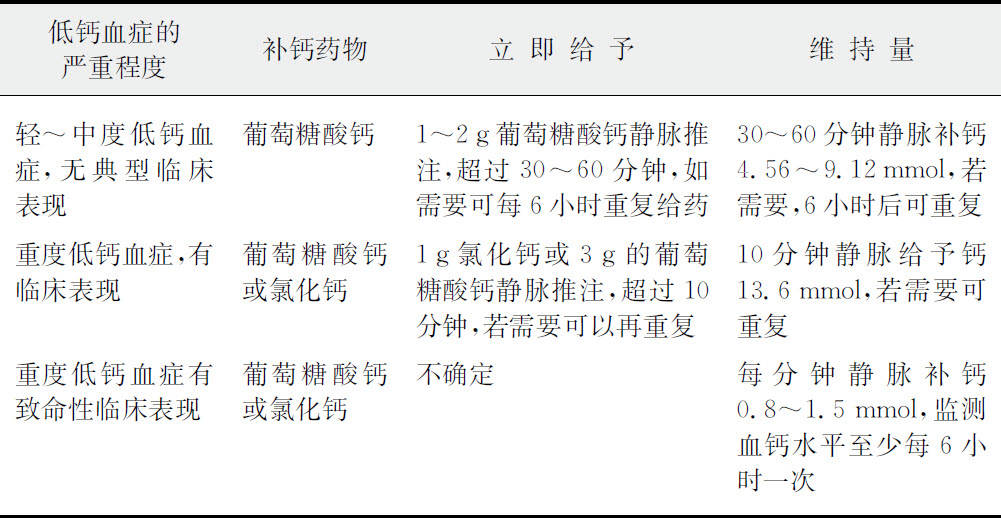
\includegraphics{./images/Image00166.jpg}
\end{table}

补钙时须注意事项:①静脉补钙最大速度为1.5mmol/分钟。②氯化钙最好从中心静脉给予,以避免外渗和局部组织坏死。③1g的氯化钙中含钙13.6mmol,1g葡萄糖酸钙中含钙4.56mmol。④注意监测血清钙水平,防止出现高钙血症。

\subsubsection{高钙血症的病因与发病机制有哪些?}

血清钙高于2.75mmol/L称为高钙血症,高钙血症的病因与发病机制为:

(1)骨质溶解增加 甲状旁腺功能亢进,甲状旁腺激素分泌增多,促进破骨细胞活性,使骨钙释放增加;骨转移性恶性肿瘤可直接破坏骨质,使骨钙释放,非骨转移性恶性肿瘤可能是由于肿瘤细胞释放甲状旁腺激素样多肽,具有生物活性而导致骨钙释放。

(2)肠黏膜吸收钙增加 维生素D中毒时,过量的维生素D一方面使肠黏膜吸收钙增加,血钙增高;另一方面导致骨组织破骨活跃,骨钙释放,血钙增高
\protect\hyperlink{text00025.htmlux5cux23ch5-24}{\textsuperscript{{[}5{]}}}
。

\subsubsection{低磷血症的原因与发病机制有哪些?}

低磷血症的原因主要为磷的再分布、摄入减少和排出增加。

(1)磷的再分布 重症患者大多数低磷血症的原因为胰岛素及葡萄糖的注射或急性过度通气。血磷急剧降低最显著的例子见于糖尿病酮症酸中毒的治疗和再喂养综合征。糖尿病酮症酸中毒与治疗前由溶质利尿造成的细胞外磷丢失有关。注射胰岛素会导致葡萄糖和磷转移入细胞内,产生低磷血症。长期营养不良者,包括酒精中毒者,在肠内外再喂养期间血磷的显著下降反映了由摄入不足而导致的细胞外低磷,并伴有葡萄糖输注后导致其快速移动到细胞内。

呼吸性碱中毒也会引起细胞外磷转移入细胞内。这是由于高pH的环境下,糖酵解酶磷酸果糖激酶的活性提高所致。在水杨酸中毒、脓毒症和肝性脑病中所见到的低磷血症可能是继发于过度通气。

(2)磷摄入减少 磷摄入减少导致低磷血症通常是一个慢性过程,并且主要见于先前存在导致钙磷和维生素D摄入减少的基础疾病的重症患者。另外,抑酸药和特定的磷酸盐结合化合物在胃肠道中与磷的结合阻止磷的吸收,也可导致低磷血症,特别是当食物中磷的含量较少时。但大多数食物富含充足的磷,低磷饮食仅见于完全禁食者。

(3)磷的排出增加 肾小管磷的排出量增加是低磷血症最常见的原因,主要见于亚临床甲状旁腺功能亢进患者。在重症患者中,由于溶质利尿、乙酰唑胺和碳酸酐酶抑制剂的应用,导致经肾磷的排出量增加。代谢性酸中毒使无机磷酸盐释放到细胞外增加,导致肾小管磷的排出量的增加,但是这不是低磷血症的常见原因,因为磷很容易从细胞内的储存中被动员。血液透析对磷的清除相对无效,因此低磷血症通常不是肾替代治疗的并发症。

\subsubsection{低磷血症如何防治?}

轻中度低磷血症通常无症状。当低磷血症严重时(血磷低于1.0mg/dl),患者可感到肌无力。通常骨骼肌和心肌首先受累,可表现为呼吸肌肌力降低,患者可能难以脱离机械通气,或者出现充血性心力衰竭的症状和体征。横纹肌溶解和溶血为严重低磷血症的少见特征。白细胞功能障碍虽不常见,但一旦发生易导致感染。另外可出现血小板功能障碍导致出血。

低磷血症也可产生中枢神经系统功能障碍。临床表现主要包括精神状况的改变、癫痫发作和神经病变。病变可能与低磷血症的直接效应有关,也可能与低磷血症导致的中枢系统氧输送减少有关。

低磷血症可导致氧输送降低、胰岛素抵抗、高氯性酸中毒及其他糖尿病酮症酸中毒并发症。因此,需重视低磷血症的治疗。血磷浓度低于1~1.5mg/dl时,需要立即处理,尤其是肌无力累及呼吸肌导致呼吸衰竭时。

由于元素磷和磷酸盐的浓度和含量的表示方法不同,对于补磷的推荐用量常常很混乱。在生理pH条件下,无机磷酸盐阴离子几乎全部以单价(\ce{H2PO4^-}
)和二价(\ce{HPO4^2-}
)的形式存在。磷补充量的计算应该以元素磷的毫克数或磷和磷酸盐的毫摩尔数为基础。一毫摩尔磷酸盐或磷原子与31mg的磷元素相等。

静脉应用的磷酸盐通常是磷酸钠或磷酸钾,适宜浓度为每毫升93毫克磷(3mmol/ml)。磷的输注量很难估计,因为体内总的磷含量由于重新分布可能并没有下降,并且治疗过程中磷酸盐的迅速转移可能使情况缓解或更加严重。因此,在补磷过程中必须密切关注血磷和其他电解质的变化,当磷酸盐以钾盐的形式被输注时尤其应当注意。

严重的低磷血症(血磷低于1.0mg/dl),每千克体重补充5~7mg磷,溶于1L5%葡萄糖溶液中输注,输注时间4~6小时以上。对于60kg体重的成人,1L输液中大约需要400mg磷或4ml磷酸钠或磷酸钾溶液(3mmol/ml);或1L5%葡萄糖溶液中加入1g磷[10ml磷酸钠或磷酸钾溶液(3mmol/ml)],输注时间12~24小时以上。较轻的低磷血症时,每千克体重补充2~4mg磷。口服补液可选择磷酸钾或者磷酸钠与磷酸钾的混合物。

低磷血症的预防很重要。在静脉输注葡萄糖的患者中,需要考虑到磷的补充。接受肠外高营养的成年患者,每天大约需要补充1g磷,或每1000kcal的能量约补充12mmol(372mg)磷。由于在胰岛素治疗过程中易发生低磷血症,糖尿病酮症酸中毒患者治疗过程中须常规补磷。

\subsubsection{高磷血症的原因和发病机制是什么?}

高磷血症由磷的排出能力受损或者细胞外磷的补充量增加所致,多见于慢性肾功能不全、磷排出能力下降的患者。重症患者严重的高磷血症则多由于细胞内磷向细胞外转移所致。

(1)磷酸盐排出受损 细胞内含有大量的磷,骨骼中同样储存有大量的磷,但细胞外磷的含量很少。正常细胞循环释放数量稳定的磷进入细胞外隙,再被收回到细胞或骨内,或经肾脏排出。排出受损主要由慢性肾功能不全所致,由于甲状旁腺激素可促进磷酸盐经肾排出,故而甲状旁腺功能减退可降低磷的经肾排出,即使此时肾功能是正常的。

(2)磷的再分布 重症患者发生高磷血症的一个常见的、特有原因为大片组织破坏,导致磷的“再分布”异常,即大量的细胞内磷向细胞外隙转移。重症患者最常见的组织损伤形式是由创伤引起的横纹肌溶解,或者由感染、药物、癫痫发作、代谢所致的其他肌肉损伤。由缺血引起的肠坏死也可导致高磷酸血症。肾功能不全可加重由磷的再分布引起的高磷血症。由于胰岛素和葡萄糖可以促进磷进入细胞内,因此患糖尿病伴胰岛素缺乏者可能更易发生高磷血症。

(3)过度补磷 低磷血症患者过度补磷可能导致高磷血症。导致这种情况出现的因素包括肾功能不全,以及低磷血症的原因被纠正后继续补磷。对于接受完全肠外营养的患者应予以密切监测,因为每升标准溶液可能含有300~500mg磷。灌肠或X线检查、结肠镜检查前口服的肠道准备药物,可能含有大量的磷酸钠作为渗透剂,如果磷酸盐被吸收,就会出现严重的高磷血症(血磷>20mg/dl)和阴离子间隙性代谢性酸中毒。

\subsubsection{高磷血症有哪些临床表现?如何治疗?}

大多数有轻中度高磷血症的患者无症状。如果钙磷乘积>60,在不同器官(包括心脏、肺及肾脏)中异位钙化的风险会增加。磷酸钙沉积所致的急性病例,主要局限于对心脏传导系统的影响,如心脏传导阻滞。

急性高磷血症也可能导致低钙血症,出现手足搐搦、癫痫发作、心律失常和低血压。治疗低磷血症和高磷血症的过程中均应检测血钙。低钙血症的产生与磷酸钙的沉积和维生素D激活所必须的肾脏1α-羟化酶抑制有关。

单纯血磷浓度升高并不需要立即处理。如有心脏传导功能紊乱(如心脏传导阻滞)或有症状的、严重的低钙血症,则需要迅速处理。治疗低钙合并高磷血症时应该降低血磷浓度而不是补钙,因为补钙可能加重异位钙化。常用的治疗方法包括:

(1)促进尿中磷排出 肾脏磷的排出有赖于适当的肾小球滤过率。因为磷酸盐的重吸收依赖于近端小管钠的重吸收,输入普通的含盐溶液可以增加磷的排泄,前提是患者可以耐受这种治疗。存在细胞外容量增加者、充血性心力衰竭和肾功能不全的患者应避免采用这种治疗方法。

(2)血液透析 此举有利于清除细胞外磷,但由于细胞外液中磷所占的比例很小,故而作用效果很短暂。碳酸钙可提高钙磷乘积,应当避免用于急性高磷酸血症的患者。紧急时可使用不含钙、不含铝的磷酸盐结合物。

(3)降低磷的摄入量 停止外源性磷的摄入,包括停止经完全肠外营养、口服或静脉磷的摄入或输注。饮食中的磷可通过低蛋白饮食、避免摄入含钙和磷的卤制品来控制到最低水平。

\subsection{镁的代谢}

\subsubsection{为什么镁代谢紊乱经常被忽略?}

镁的代谢及功能与钙、磷有密切关系。人体含镁量20~28g,一半以上存在于骨中,其余在细胞内,是细胞内重要的阳离子之一。细胞外液中的镁不超过体内总镁量的1%。镁与人类许多生理功能密切相关,在疾病发生及临床治疗中有重要作用。骨中镁主要以Mg\textsubscript{3}
(PO\textsubscript{4} )\textsubscript{2} 和MgCO\textsubscript{3}
的形式存在,吸附于羟磷石表面。但它与钙不同,不易随机体需要从骨中动员出来,但镁在一定程度上可置换骨中的钙,其置换的量取决于骨钙动员的状况。正常人血镁约1/3与血浆蛋白(主要是白蛋白)结合,少部分与磷酸、柠檬酸等结合成不易解离的化合物,而绝大部分(约60%)以Mg\textsuperscript{2+}
形式存在。细胞内镁则大部分与磷酸根、柠檬酸根及其他阴离子结合为复合物,尤其是与ATP结合为Mg-ATP形式,参与需要ATP的反应。

人体每日镁的需要量为0.2~0.4g,主要从绿色蔬菜中获得。镁的吸收主要在小肠,膳食中磷酸盐和乳糖的含量、肠腔内镁的浓度及肠道功能状态均影响镁的吸收。维生素D对肠道镁的吸收有轻微的促进作用。钙与镁的吸收有竞争作用。因此,食物中含钙过多则妨碍镁的吸收。镁的排泄主要是通过肠道和肾脏,60%~70%的镁从粪便排出,血浆中的镁离子可透过肾小球滤出,大部分可被肾小管重吸收,只有2%~10%随尿排出。缺镁则肾小管重吸收加强。甲状腺素促进镁的排泄。

镁是许多酶系的辅助因子或激活剂,广泛参与体内各种物质代谢,包括蛋白质、脂肪、糖及核酸的代谢。镁离子对神经系统和心肌作用十分重要,对中枢神经系统和神经肌肉接头,镁离子能起到镇静和抑制作用:

\[
\text{神经肌肉应激性}\propto    \frac{[\ce{Na+}]+[\ce{K+}]}{[\ce{Ca^2+}]+[\ce{Mg^2+}]+[\ce{H+}]}
\]

对于神经肌肉应激性,镁离子与钙离子是协同的,但对于心肌钙离子与镁离子的作用又是相互拮抗的:

\[
\text{心肌应激性}\propto    \frac{[\ce{Na+}]+[\ce{Ca^2+}]}{[\ce{K+}]+[\ce{Mg^2+}]+[\ce{H+}]}
\]

因此,低血镁可引起与低血钙类似的手足搐搦症,而镁中毒则可导致四肢软弱无力及心律不齐等。镁作用于外周血管可引起血管扩张,血清镁离子浓度对甲状旁腺素和降钙素的分泌均有影响。血清镁离子浓度过低,则PTH分泌受抑制,而不再受钙离子的调节。因此,可出现低血钙与低血镁并存的情况。新生儿低血钙亦往往伴有低血镁,单独给予镁剂,则血镁和血钙均可升高。此外,低血镁还可影响甲状旁腺素对靶细胞的作用,此时给予外源性甲状旁腺素亦不起反应。高血镁可刺激降钙素的分泌,结果可出现低血钙与高血镁并存的情况。但由于长期以来临床医生对镁代谢异常认识不足或未进行常规监测,故镁的异常经常被忽略。

血清镁含量低于0.75mmol/L称为低镁血症。血清镁浓度高于1.25mmol/L称为高镁血症。严重的低镁血症主要引起神经肌肉系统症状。包括呼吸肌乏力、精神症状、反射亢进,甚至可以看到像低钙血症时的手足抽搐。低镁血症可以发生室性心律失常和充血性心衰。但临床上因低镁血症导致的室性心律失常常易被忽视。

高镁血症主要表现为中枢神经系统和神经肌肉系统症状,精神症状、昏睡、深部腱反射减弱和软弱麻痹是高镁血症的主要临床特点。

\subsubsection{为何外科术后的患者易导致低镁血症?}

外科危重患者术后可因多种因素导致镁的丢失,加之临床上常忽视镁的补充及对缺镁的临床表现认识不足,不能及时补充镁,从而发生低镁血症。

低镁血症的原因包括:①术前进食少或禁食、呕吐,从术前、术后胃管、腹腔引流管、胆道T形管丢失大量水、电解质(包括镁)而未及时补充,胃癌伴幽门梗阻患者术前虽补充但剂量不足。②坏死性出血性胰腺炎及惠普尔术后胰瘘患者,由于脂肪皂化,镁及钙与脂肪酸结合成脂肪镁、脂肪钙沉积于受损害的胰腺及周围组织中,导致低血镁。③危重患者因感染中毒、高胆红素血症、多种毒素及有害物质损伤肾小管引起尿镁的再吸收减少,排出增加。④胰岛素促使镁进入肌细胞而产生低镁血症。⑤反复使用洋地黄、利尿药可明显增加钾、镁、钙的排泄,导致药源性低镁血症。

\subsubsection{低镁血症主要危害有哪些?}

镁是人体中重要的金属离子,对维持正常的生理功能有重要作用。在人体内除了Ca\textsuperscript{2+}
、K\textsuperscript{+} 、Na\textsuperscript{+}
外,Mg\textsuperscript{2+}
居金属元素含量的第4位,是细胞内仅次于K\textsuperscript{+}
的第二大阳离子。镁离子是300多种酶的辅助因子,特别是在调整能量代谢和跨膜电位活动方面起着重要作用。镁可以维持细胞内外离子的通透性,同时镁作为钙离子的“天然”拮抗剂,可抑制钙离子内流,因此,在低镁或者补镁时,可影响心脏电生理特性,导致心律失常。

低镁血症主要的病理生理变化包括:①在低镁时,钠钾泵活性降低,使细胞内失钾,引起静息膜电位降低,心肌兴奋性增加,传导减慢;②镁对慢通道离子流有阻滞作用,缺镁时,钙离子经慢通道进入细胞速度加快,使动作电位曲线平台期缩短,有效不应期也缩短,传导减慢及不应期缩短均有利于折返;③缺镁时自律细胞的除极加快,自律性增高;④低镁可引起儿茶酚胺过多,导致心律失常,尤其是室性心律失常,典型表现为尖端扭转型室性心律失常,并且使室性心律失常发生的阈值降低。严重时发生室颤,甚至心跳骤停。

补充镁可使心肌自律性、兴奋性和传导性降低,有利于消除折返、自律性增高或触发活动引起的心律失常。

\subsubsection{为什么部分低钾导致的心律失常经补钾后无效?}

临床上可遇见低镁(如急性心梗)、低钾(洋地黄中毒)或低镁合并低钾(运用利尿剂)等所致的各种心律失常,特别是室性房性心动过速,单纯的低镁或低钾引起的心律失常补镁或补钾可减少或终止心律失常的发生,而低镁合并的低钾所致的心律失常单独补钾常不能纠正心律失常,因为低镁使Na\textsuperscript{+}
-K\textsuperscript{+}
-ATP酶作用减弱,因此尽管补钾后血清钾水平正常,但细胞内钾的水平仍然是低的,另外,低镁可减弱肾脏保钾作用,所以在治疗心律失常时应在监测血清钾和镁的基础上积极补充钾和镁。

\subsubsection{如何防止低镁血症?}

严重低镁血症可引起心律失常和神经肌肉系统症状,积极防止低镁血症的方法有:①要警惕临床上发生低镁血症的可能性,尤其是重症患者应尽量消除或减少各种镁缺乏的诱因。②对低血钾、低血钙患者经补钾补钙不能迅速纠正时,应及时观察血镁。③对有精神症状的重症患者,应在围手术期及时监测血清镁,并有效补充镁制剂。④减少或慎用庆大霉素、胰岛素。当各种高危因素不可避免地存在时,应定期做心电图及血镁的监测。根据镁的丢失量积极补充,原则上是补充量应大于估计的缺失量,补镁时要监测血清镁水平
\protect\hyperlink{text00025.htmlux5cux23ch6-24}{\textsuperscript{{[}6{]}}}
。

\subsubsection{为什么低镁血症患者常合并低钾、低钙血症?}

出现低镁血症时常合并低钾,原因有:①造成镁丢失的途径同样可造成钾丢失。②镁是激活细胞内Na\textsuperscript{+}
-K\textsuperscript{+}
-ATP酶所必需的离子,当镁缺乏时,其活性减退,细胞外钾内流,造成细胞外缺钾而致低钾血症。③缺镁时,肾保钾能力减低,故使血钾降低。

低血镁时也常合并低钙血症,主要是血中镁离子浓度降低常致钙从钙库游离入血发生障碍而造成低血钙。

由于镁、钾、钙三种电解质减少或比例失调,其临床表现呈多样化而不典型。因此,对于危重患者尤其是胰胆疾病及幽门梗阻术后患者,当有导致低镁的诱因时,要警惕低镁血症的发生。若患者需要肠内或肠外营养支持,应适量加入镁、钾、钙,甚至磷,以保持人体微量元素平衡。一旦出现持久而较难纠正的低血钾或经大量补钙而神经肌肉兴奋症状不见好转或加重时,要首先考虑低镁血症的可能,应及时监测血镁。

\begin{center}\rule{0.5\linewidth}{\linethickness}\end{center}

参考文献

\protect\hyperlink{text00025.htmlux5cux23ch1-24-back}{{[}1{]}} .Michael
DK,Imad FB,Gordon SS,et al.Treatment of electrolyte disorders in
adult patients in the intensive care unit.Am J Health-Syst
Pharm,2005,62:1663-1682.

\protect\hyperlink{text00025.htmlux5cux23ch2-24-back}{{[}2{]}}
.Lipworth BJ,Mcdevitt DG,Struthers AD,et al.Prior treatment with
diuretic augments the hypokalemia and electrocardiographic effects of
inhaled albuterol.Am J Med,1989,86:653-670.

\protect\hyperlink{text00025.htmlux5cux23ch3-24-back}{{[}3{]}} .Zaloga
GP,Chernow B.The multifactorial basis for hypocalcemia during
sepsis.Ann Intern Med,1987,107:36-40.

\protect\hyperlink{text00025.htmlux5cux23ch4-24-back}{{[}4{]}} .Vincent
JL,Bredas P,Jankowski S,et al.Correction of hypocalcemia in the
critically ill:What is the haemodynamic benefit?Intensive Care
Med,1995,21:838-842.

\protect\hyperlink{text00025.htmlux5cux23ch5-24-back}{{[}5{]}} .Burtis
WJ,Wu TL,Insogna KL,et al.Humoral hypercalcemia of malignancy.Ann
Intern Med,1988,108:454-459.

\protect\hyperlink{text00025.htmlux5cux23ch6-24-back}{{[}6{]}} .Chernow
B,Bamberger S,Stoiko M,et al.Hypomagnesemia in patients in
postoperative intensive care.Chest,1987,95:391-397.

\protect\hypertarget{text00026.html}{}{}

